\documentclass[journal,12pt,twocolumn]{IEEEtran}
\makeatletter
\@addtoreset{figure}{problem}
\makeatother
\usepackage{setspace}
\usepackage{gensymb}
\usepackage{xcolor}
\usepackage{caption}
\singlespacing

\usepackage[cmex10]{amsmath}
\usepackage{mathtools}
\usepackage{amsthm}
\usepackage{mathrsfs}
\usepackage{txfonts}
\usepackage{stfloats}
\usepackage{cite}
\usepackage{cases}
\usepackage{mathtools}
\usepackage{subfig}
\usepackage{longtable}
\usepackage{multirow}
\usepackage{enumitem}
\usepackage{mathtools}
\usepackage{listings}
    \usepackage[latin1]{inputenc}                                 %%
    \usepackage{color}                                            %%
    \usepackage{array}                                            %%
    \usepackage{longtable}                                        %%
    \usepackage{calc}                                             %%
    \usepackage{multirow}                                         %%
    \usepackage{hhline}                                           %%
    \usepackage{ifthen}                                           %%
    \usepackage{lscape}     
\usepackage[american]{circuitikz}
\DeclareMathOperator*{\Res}{Res}
\renewcommand\thesection{\arabic{section}}
\renewcommand\thesubsection{\thesection.\arabic{subsection}}
\renewcommand\thesubsubsection{\thesubsection.\arabic{subsubsection}}

\renewcommand\thesectiondis{\arabic{section}}
\renewcommand\thesubsectiondis{\thesectiondis.\arabic{subsection}}
\renewcommand\thesubsubsectiondis{\thesubsectiondis.\arabic{subsubsection}}
\hyphenation{op-tical net-works semi-conduc-tor}

\def\inputGnumericTable{}                                 %%
\lstset{
language=C,
frame=single, 
breaklines=true
}
 

\begin{document}
%

\theoremstyle{definition}
\newtheorem{theorem}{Theorem}[section]
\newtheorem{problem}{Problem}
\newtheorem{proposition}{Proposition}[section]
\newtheorem{lemma}{Lemma}[section]
\newtheorem{corollary}[theorem]{Corollary}
\newtheorem{example}{Example}[section]
\newtheorem{definition}{Definition}[section]
\newcommand{\BEQA}{\begin{eqnarray}}
\newcommand{\EEQA}{\end{eqnarray}}
\newcommand{\define}{\stackrel{\triangle}{=}}

\bibliographystyle{IEEEtran}
\providecommand{\nCr}[2]{\,^{#1}C_{#2}} % nCr
\providecommand{\nPr}[2]{\,^{#1}P_{#2}} % nPr
\providecommand{\mbf}{\mathbf}
\providecommand{\pr}[1]{\ensuremath{\Pr\left(#1\right)}}
\providecommand{\qfunc}[1]{\ensuremath{Q\left(#1\right)}}
\providecommand{\sbrak}[1]{\ensuremath{{}\left[#1\right]}}
\providecommand{\lsbrak}[1]{\ensuremath{{}\left[#1\right.}}
\providecommand{\rsbrak}[1]{\ensuremath{{}\left.#1\right]}}
\providecommand{\brak}[1]{\ensuremath{\left(#1\right)}}
\providecommand{\lbrak}[1]{\ensuremath{\left(#1\right.}}
\providecommand{\rbrak}[1]{\ensuremath{\left.#1\right)}}
\providecommand{\cbrak}[1]{\ensuremath{\left\{#1\right\}}}
\providecommand{\lcbrak}[1]{\ensuremath{\left\{#1\right.}}
\providecommand{\rcbrak}[1]{\ensuremath{\left.#1\right\}}}
\theoremstyle{remark}
\newtheorem{rem}{Remark}
\newcommand{\sgn}{\mathop{\mathrm{sgn}}}
\providecommand{\abs}[1]{\left\vert#1\right\vert}
\providecommand{\res}[1]{\Res\displaylimits_{#1}} 
\providecommand{\norm}[1]{\lVert#1\rVert}
\providecommand{\mtx}[1]{\mathbf{#1}}
\providecommand{\mean}[1]{E\left[ #1 \right]}
\providecommand{\fourier}{\overset{\mathcal{F}}{ \rightleftharpoons}}
%\providecommand{\hilbert}{\overset{\mathcal{H}}{ \rightleftharpoons}}
\providecommand{\system}{\overset{\mathcal{H}}{ \longleftrightarrow}}
	%\newcommand{\solution}[2]{\textbf{Solution:}{#1}}
\newcommand{\solution}{\noindent \textbf{Solution: }}
\providecommand{\dec}[2]{\ensuremath{\overset{#1}{\underset{#2}{\gtrless}}}}
\DeclarePairedDelimiter{\ceil}{\lceil}{\rceil}
%\numberwithin{equation}{subsection}
\numberwithin{equation}{problem}
%\numberwithin{problem}{subsection}
%\numberwithin{definition}{subsection}
\makeatletter
\@addtoreset{figure}{problem}
\makeatother

\let\StandardTheFigure\thefigure
%\renewcommand{\thefigure}{\theproblem.\arabic{figure}}
\renewcommand{\thefigure}{\theproblem}
\numberwithin{equation}{problem}
\numberwithin{problem}{section}
\makeatletter
\@addtoreset{table}{problem}
\makeatother

\let\StandardTheFigure\thefigure
\let\StandardTheTable\thetable

\def\putbox#1#2#3{\makebox[0in][l]{\makebox[#1][l]{}\raisebox{\baselineskip}[0in][0in]{\raisebox{#2}[0in][0in]{#3}}}}
     \def\rightbox#1{\makebox[0in][r]{#1}}
     \def\centbox#1{\makebox[0in]{#1}}
     \def\topbox#1{\raisebox{-\baselineskip}[0in][0in]{#1}}
     \def\midbox#1{\raisebox{-0.5\baselineskip}[0in][0in]{#1}}

\vspace{3cm}

\title{ 
	\logo{Motion Repeater implementation on UGV}
}
 \author{G V V Sharma$^{*}$% <-this % stops a space
 \thanks{*The author is with the Department
 of Electrical Engineering, Indian Institute of Technology, Hyderabad
 502285 India e-mail:  gadepall@iith.ac.in. All content in this manual is released under GNU GPL. Free and open source.}% <-this % stops a space
}
\maketitle

\tableofcontents

\bigskip

\begin{abstract}
This manual is for making UGV repeat the motion  
\end{abstract}
\IEEEpeerreviewmaketitle

\section{Hardware setup}
Build the toycar refering the manual in the below link
\begin{lstlisting}
https://github.com/gadepall/ugv/tree/main/manual
\end{lstlisting}
% \input{./figs/specs.tex}
\section{Software setup}
Flash the code available in below link of the platformio project 
\begin{lstlisting}
https://github.com/Hruday-Beeravelli/UGV-Project/tree/main/UGV-Motion-Repeat1
\end{lstlisting}
either using VSCode or using command line
\begin{lstlisting}
pio run
\end{lstlisting}
for compiling the code
\begin{lstlisting}
pio run -t nobuild -t upload
\end{lstlisting}
for uploading the code into esp32
\section{Circuit setup}
Connect the componets based on the diagram Fig \ref{fig:circuit}
\begin{center}
\begin{figure}[!ht]
    \centering
    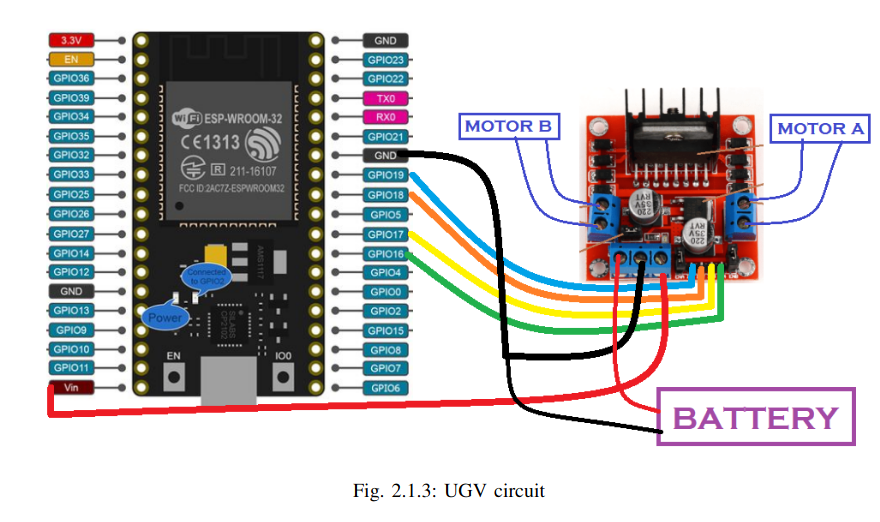
\includegraphics[width=\columnwidth]{circuit.png}
    \caption{}
    \label{fig:circuit}
\end{figure}
\end{center}
\section{Controlling}
Install ``Arduino \& ESP32 Bluetooth Controller App - Dabble" from 
\begin{lstlisting}
  https://play.google.com/store/apps/details?id=io.dabbleapp
\end{lstlisting}
% \begin{center}
connect to ESP32 by clicking the unplugged button on top right corner, and selecting bluetooth name. find the similar interface like in fig \ref{fig:repeat} by clicking GamePad. and use the buttons accordingly by refering to table
\begin{table}[]
    \centering
    \caption{Dabble buttons and their functions}
    \begin{tabular}{ |m{1.5cm}| m{15.8em} |}

 \hline
 \textbf{Button} &  \textbf{Funtion} \\ [1ex] 
 \hline\hline
 1 & Forward\\
 \hline
 2 & Left\\
 \hline
 3 & Backward\\
 \hline
 4 & Right\\
 \hline
 5 & Starts Motion from recorded sample\\  
 \hline
 6 & Starts Recording the inputs and duriation\\ 
 \hline
 7 & Stops recording the inputs \\ [0.5ex]
 \hline
 
\end{tabular}
\label{tab:1}
    
\end{table}
% \end{center}
\renewcommand{\thetable}{\theproblem}

\begin{center}
\begin{figure}[!ht]
    \centering
    \includegraphics[width=\columnwidth]{repeater.png}
    \caption{}
    \label{fig:repeat}
\end{figure}
\end{center}

\end{document}
